\chapter{System Design}
% Provide a detailed explanation of the overall system architecture
% \cite{lin1991divergence}, i.e. the HOW of the project.
% Use UML, system architecture diagrams, screenshots, code snippets 
% and algorithms to illustrate your design.

\section{Client}
Python files with the $frame.py$ suffix contain Tkinter frame classes.

\section{Server Dashboard}
The dashboard is a single-page web application (SPA) it is fully written in JavaScript.
And doesn't make use of any external libraries.
I made this decision early because I wanted to keep the project as self-contained as possible.

The dashboard is object-oriented, all of the main code can be found in the \textbf{server/static/js/index.js} file.
This contains code for communicating with the server endpoints and classes for each page.

All pages inherit the \textbf{Page} class, as they share common functionality which upholds the DRY principle.


Each page class must implement the \textbf{loadPage} method, which is called when the page is loaded.
This can be used for fetching data from the backend.



\section{Server Endpoints}
The server uses the flask micro-framework to provide the RESTful API.
I decided to categorise the API into five sections: clients, databases, patterns, tasks and workers.
Flask supports a feature called blueprints, which allows you to split your web application into multiple components.
I used a blueprint for each of the five sections of the API, and each blueprint is stored in a separate file.

This is an example of a blueprint taken from the worker's blueprint.
\begin{lstlisting}[language=python]
...

import flask

...

workers = flask.Blueprint(__name__, "workers")

@workers.get("/api/workers")
def get_records_route():
    return database.get_caladium_collection("workers")

...
\end{lstlisting}

\section{Sandbox}



% architecture.png
\begin{figure}[h!]
    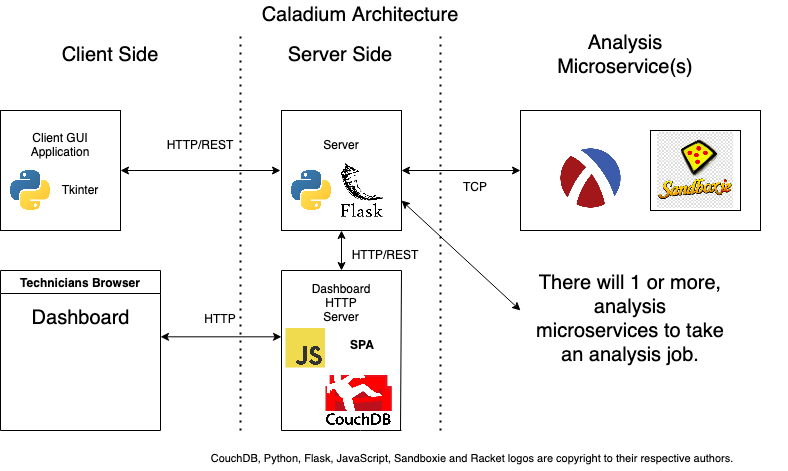
\includegraphics[width=0.9\textwidth]{images/architecture.png}
    \caption{System Architecture.}
    \label{image:sysArchitecture}
\end{figure}



\section{Working with Images}
You can embed an image in a \LaTeX document using the technique shown below. System diagrams and images with a small number of colours (100s, not 1000s) should be stored in PNG format. Although \LaTeX doesn't care where you place your images, it is good practice to place them in a single sensible directory and apply some sort of hierarchy to them, e.g. the path images/chapter 1 might contain all of the images for Chapter 1 of your dissertation.

\begin{figure}[h!]
    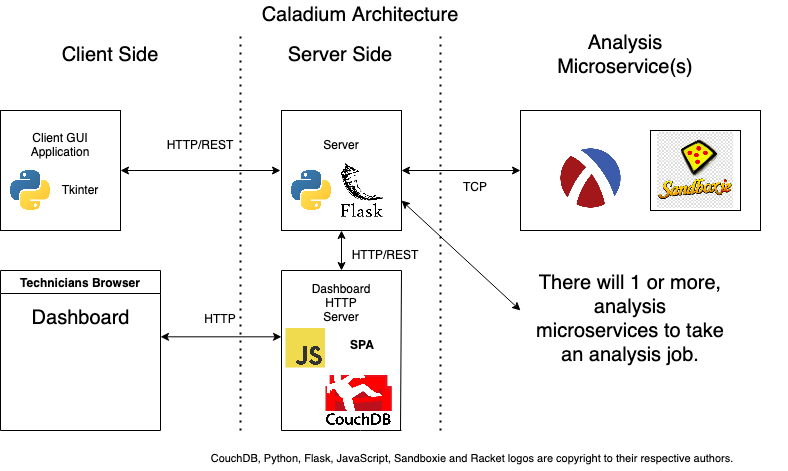
\includegraphics[width=0.9\textwidth]{images/architecture.png}
    \caption{System Architecture.}
    \label{image:sysArchitecture}
\end{figure}

Image \ref{image:sysArchitecture} can be referenced with the label given to the image, \\ i.e. \textbf{\textbackslash{}ref\{image:sysArchitecture\}}. Note that \LaTeX will place the image wherever it deems fit. Don't bother trying to change where a table or figure is placed until your document is ready for the final layout.
